\section{Geomagic touch}\label{sec:geo_magic}
The Geomagic Touch(GT) is a haptic feedback device, which has the ability to manipulate its joints in such a way that the user feels resistance when moving the pin in a certain direction or way. The Geomagic Touch described in this section can be seen on \figref{fig:phantom_omni}.

\begin{figure}[H]
	\centering
	\begin{subfigure}{.45\textwidth}
		\centering
		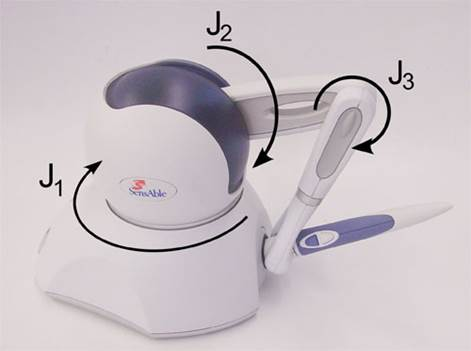
\includegraphics[width=\linewidth]{haptick1.png}
		\caption{Overview of the Geomagic Touch's first three joints.}
		\label{fig:phantom1}
	\end{subfigure}
	\begin{subfigure}{.45\textwidth}
		\centering
		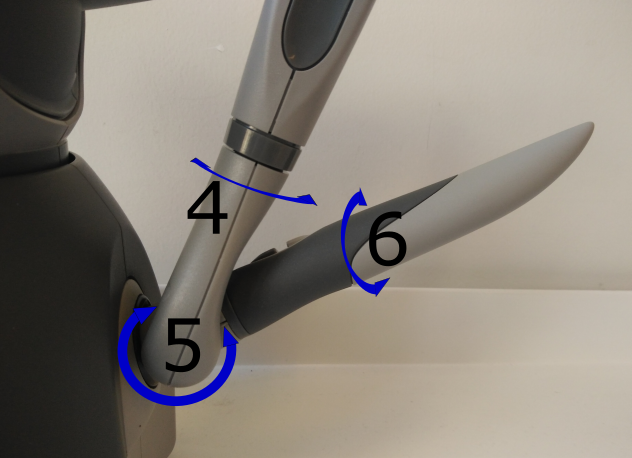
\includegraphics[width=\linewidth,height=5.4cm]{haptick2.png}
		\caption{Overview of the Geomagic Touch's last three joint}
		\label{fig:phantom2}
	\end{subfigure}
\caption{Overview of all the Geomagic Touch's joints.}
\label{fig:phantom_omni}
\end{figure}

As mentioned the Geomagic Touch has the ability to generate resistance for the user. In other words, when moved in a specific direction it can create a counter force in respect to a certain position. On \figref{fig:phantom_omni}, it can be seen that the omni has six \gls{DOF}, where only the first three can be actuated, see \figref{fig:phantom1}. This means that the device only has the ability to generate force feedback with three \gls{DOF}, in this case roll, pitch and yaw.

The connection to the Geomagic Touch can either be made directly through a ethernet cable or through ethernet cable to a usb converter into a computer. For programming the omni an API is included, which enables the connection to the GT. The GT has a lot of features which can be programmed through the language C++, e.g force rendering or drawing graphics.
